\section{IMU Residual Covariance}
\label{sec:maci2:imu_residual_cov}

The covariance of the IMU residual can be derived from the IMU preintegration covariance:
\begin{equation}
\begin{aligned}
\Sigma^r_{\gamma_k} &= J_r^{-1}(\mathbf{r}_{\gamma_k}) \Sigma^{\Delta R}_k (J_r^{-1}(\mathbf{r}_{\gamma_k}))^T, \\
\Sigma^v_{\beta_k} &= \Sigma^{\Delta v}_k, \\
\Sigma^p_{\alpha_k} &= \Sigma^{\Delta p}_k,
\end{aligned}
\end{equation}
The computed covariance can then be used in our tuning-free optimization.


\section{Learned IMU Model}
\label{sec:maci2:learned_imu_model}

\begin{figure}[htbp]
\centering
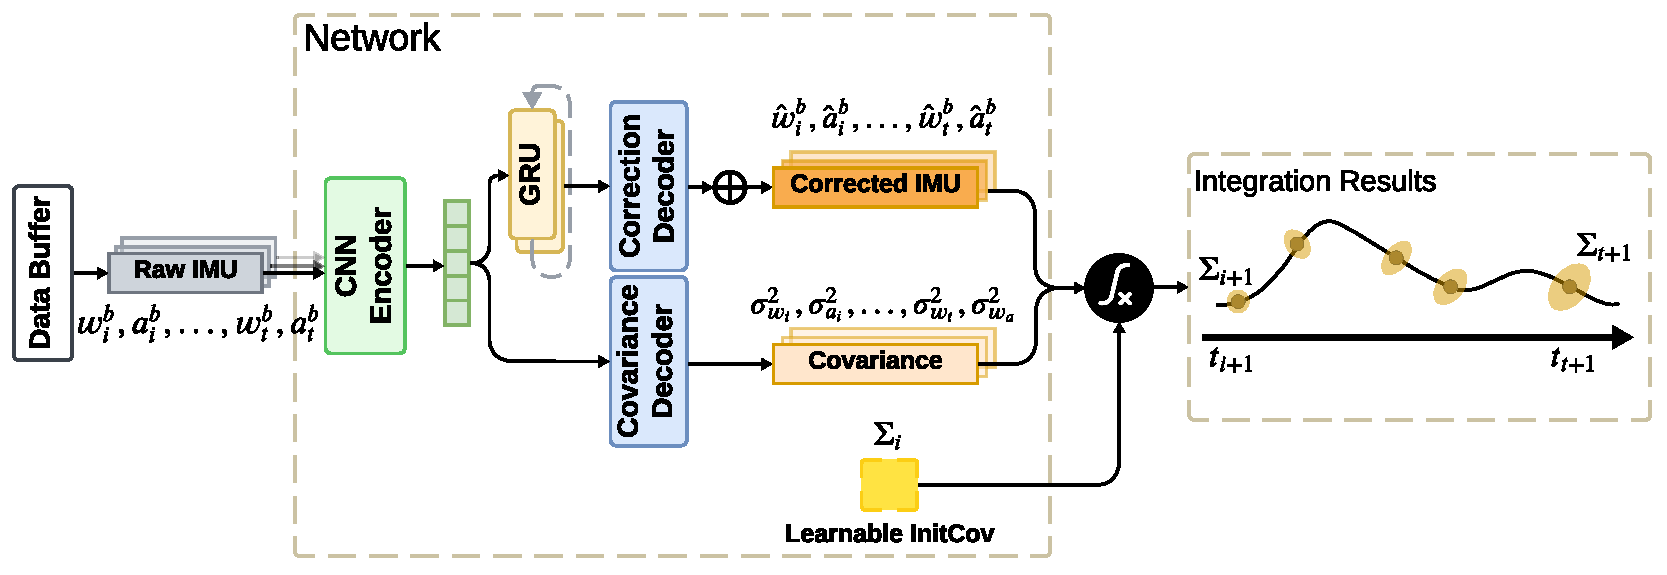
\includegraphics[width=0.8\columnwidth]{tex/ch6_macinit/figs/system_pipeline - AirIMU_new.pdf}
\caption{Network architecture of the learned IMU model developed in this chapter.}
\label{fig:maci2:airimu_net}
\end{figure}

\noindent \textbf{Network Architecture.} The network architecture of the learned IMU model is illustrated in \fref{fig:maci2:airimu_net}. Following AirIMU, we train a shared CNN encoder network to leverage the hidden relationship between IMU correction and uncertainty, while we do not use GRU-processed data to predict the uncertainty. In addition, a learnable initial covariance is introduced.

\noindent \textbf{IMU Preintegration Covariance Propagation.} Our model jointly supervises the integrated IMU state and the propagated covariance to train the model. The preintegration covariance propagation is as follows:
\begin{equation}
\label{eq:maci2:cov_prop_appendix}
\begin{aligned}
\bm{\Sigma}_{ik+1} &= \mathbf{A}\bm{\Sigma}_{ik}\mathbf{A}^T + \mathbf{B}\text{diag}(\bm{\Sigma}^{gyro}, \bm{\Sigma}^{acc})\mathbf{B}^T \\
&= \mathbf{A}\bm{\Sigma}_{ik}\mathbf{A}^T + \mathbf{B}_g\bm{\Sigma}^{gyro}\mathbf{B}_g^T + \mathbf{B}_a\bm{\Sigma}^{acc}\mathbf{B}_a^T,
\end{aligned}
\end{equation}
where $\bm{\Sigma}^{gyro}$ and $\bm{\Sigma}^{acc}$ are the measurement covariance, which is obtained with the uncertainty prediction of the network. The propagation starts from $\bm{\Sigma}_{ii} = \bm{\Sigma}_{0}$, where $\bm{\Sigma}_{0}$ is the learned initial covariance. $\mathbf{A}$ and $\mathbf{B}$ can be computed by:
\begin{equation}
\begin{aligned}
A &= \begin{bmatrix}
\Delta R_{kk+1}^T & 0_{3 \times 3} & 0_{3 \times 3} \\
-\Delta R_{ik}(a_k^{\wedge})\Delta t & I_{3 \times 3} & 0_{3 \times 3} \\
-1/2\Delta R_{ik}(a_k^{\wedge})\Delta t^2 & I_{3 \times 3}\Delta t & I_{3 \times 3}
\end{bmatrix},\\
B &= [B_g, B_a], \\
B_g &= \begin{bmatrix}
J_r^k\Delta t \\
0_{3 \times 3} \\
0_{3 \times 3}
\end{bmatrix}, \quad B_a = \begin{bmatrix}
0_{3 \times 3} \\
\Delta R_{ik}\Delta t \\
1/2\Delta R_{ik}\Delta t^2
\end{bmatrix},
\end{aligned}
\end{equation}
$\cdot^{\wedge}$ denotes the skew matrix, $\Sigma \in R^{9\times 9}$ is the covariance matrix of the IMU preintegration term. $\Sigma^{gyro}$ and $\Sigma^{acc}$ are the measurement covariance, which is obtained with the uncertainty prediction of the network. $J_r^k$ is the right Jacobian of $SO(3)$ evaluated with the integrated rotation at the $k$-th time step.

\noindent\textbf{Training Losses.} Given the IMU preintegration terms $\bm{\gamma}^{b_i}_{b_j}, \bm{\beta}^{b_i}_{b_j}, \bm{\alpha}^{b_i}_{b_j}$ from frame $b_i$ to $b_j$, the $j$-th state of the robot in the world frame $\{W\}$ can be computed by:
\begin{equation}
\label{eq:maci2:world_inte}
\begin{aligned}
\mathbf{q}^{w}_{b_j} &= \mathbf{q}^{w}_{b_i} \bm{\gamma}_{b_j}^{b_i}, \\
\mathbf{v}_{b_j}^{w} &= \mathbf{v}_{b_i}^{w} + \mathbf{g}^{w} \Delta t_{ij} + \mathbf{R}^{w}_{b_i} \bm{\beta}_{b_j}^{b_i}, \\
\mathbf{p}^{w}_{b_{j}} &= \mathbf{p}^{w}_{b_i} + \mathbf{v}^{w}_{b_i} \Delta t_{ij} + \frac{1}{2} \mathbf{g}^{w} \Delta t_{ij}^2 + \mathbf{R}^{w}_{b_i} \bm{\alpha}_{b_j}^{b_i},
\end{aligned}
\end{equation}

The correction loss is then designed as:
\begin{equation}
\begin{aligned}
L_r &= \| \text{Log}(\hat{\mathbf{q}}_w^{b_i} \mathbf{q}^w_{b_i}) \|_h, \\
L_v  &= \| \mathbf{v}^{w}_{bi}-\hat{\mathbf{v}}^{w}_{bi} \|_h, \\
L_p  &= \| \mathbf{p}^{w}_{bi}-\hat{\mathbf{p}}^{w}_{bi} \|_h,
\end{aligned}
\end{equation}
where $\hat{\mathbf{q}}_w^{b_i}$, $\hat{\mathbf{v}}^{w}_{bi}$, and $\hat{\mathbf{p}}^{w}_{bi}$ are ground truth. The $\|\cdot\|_h$ denotes the Huber function.

The covariance loss is designed as:
\begin{equation}
\begin{aligned}
L_r^{cov} &=\frac{1}{2} (\| \text{Log}(\hat{\mathbf{q}}_w^{b_j} \mathbf{q}^w_{b_j}) \|^2_{\Sigma^r_{i,j}} + \text{ln}(\det(\Sigma^r_{i,j}))),\\
L_v^{cov}  &= \frac{1}{2} (\| \mathbf{v}^{w}_{bj}-\hat{\mathbf{v}}^{w}_{bj} \|^2_{\Sigma^v_{i,j}} + \text{ln}(\det(\Sigma^v_{i,j}))), \\
L_p^{cov}  &= \frac{1}{2} (\| \mathbf{p}^{w}_{bj}-\hat{\mathbf{p}}^{w}_{bj} \|^2_{\Sigma^p_{i,j}} + \text{ln}(\det(\Sigma^p_{i,j}))),
\end{aligned}
\end{equation}
where $\Sigma^r_{i,j}$, $\Sigma^v_{i,j}$, $\Sigma^p_{i,j}$ can be computed from the IMU preintegration covariances $\Sigma^{\Delta}_{i,j}$:
\begin{equation}
\begin{aligned}
\Sigma^r_{i,j} &= J_r^{-1}(\text{Log}(\hat{\mathbf{q}}_w^{b_j} \mathbf{q}^w_{b_j})) \Sigma^{\Delta R}_{i,j} J_r^{-1}(\text{Log}(\hat{\mathbf{q}}_w^{b_j} \mathbf{q}^w_{b_j}))^T, \\
\Sigma^v_{i,j} &= \mathbf{R}^w_{b_i} \Sigma^{\Delta v}_{i,j} (\mathbf{R}^w_{b_i})^T, \\
\Sigma^p_{i,j} &= \mathbf{R}^w_{b_i} \Sigma^{\Delta p}_{i,j} (\mathbf{R}^w_{b_i})^T.
\end{aligned}
\end{equation}


\section{Analytical Jacobians}
\label{sec:maci2:jacobians}

This section summarizes the analytical Jacobians used throughout our optimization. We linearize all residuals on $\operatorname{SO}(3)$ and $\operatorname{SE}(3)$ using a left-multiplicative perturbation model and report derivatives with respect to minimal tangent-space coordinates.

\subsection{Notation}

\paragraph{$\operatorname{SE}(3)$ exponential/logarithm.}
For $\boldsymbol{\xi}=\begin{bmatrix}\boldsymbol{\phi}^\top & \boldsymbol{\rho}^\top\end{bmatrix}^\top\in\mathbb{R}^6$
we use $\text{Exp}:\mathbb{R}^6\!\to\!\operatorname{SE}(3)$ and $\text{Log}:\operatorname{SE}(3)\!\to\!\mathbb{R}^6$ with standard Lie definitions.
We denote the \emph{right/left Jacobians} on $\operatorname{SE}(3)$ by
$\mathbf{J}_r(\boldsymbol{\xi}),\mathbf{J}_l(\boldsymbol{\xi})\in\mathbb{R}^{6\times 6}$ and their inverses
$\mathbf{J}_r^{-1},\mathbf{J}_l^{-1}$.

\paragraph{Adjoint of $\operatorname{SE}(3)$.}
For $\mathbf{T}=(\mathbf{R},\mathbf{p})\in\operatorname{SE}(3)$, the adjoint $\mathrm{Ad}_{\mathbf{T}}\in\mathbb{R}^{6\times 6}$ acting on
$\boldsymbol{\xi}=\begin{bmatrix}\boldsymbol{\phi}\\\boldsymbol{\rho}\end{bmatrix}$ (rotation first) is
\begin{equation}
\begin{aligned}
\mathrm{Ad}_{\mathbf{T}} \triangleq {}&
\begin{bmatrix}
\mathbf{R} & \mathbf{0}\\
[\mathbf{p}]_\times \mathbf{R} & \mathbf{R}
\end{bmatrix},\\
\mathrm{Ad}_{\mathbf{T}}
\begin{bmatrix}\boldsymbol{\phi}\\\boldsymbol{\rho}\end{bmatrix}
:={}&
\begin{bmatrix}
\mathbf{R}\boldsymbol{\phi}\\
[\mathbf{p}]_\times \mathbf{R}\boldsymbol{\phi}+\mathbf{R}\boldsymbol{\rho}
\end{bmatrix}.
\end{aligned}
\end{equation}

\subsection{Left Perturbation Model}

The optimization variables include (\eref{eq:maci2:state}):
\begin{equation}
\begin{aligned}
\mathbf{T}_{c0}^{b_k}
&=
\begin{bmatrix}
\mathbf{R}_{c0}^{b_k} & \mathbf{p}_{c0}^{b_k}\\
\mathbf{0}^\top & 1
\end{bmatrix}\in\operatorname{SE}(3),\\
\mathbf{v}_{b_k}^{b_k} &\in\mathbb{R}^3,\qquad
\mathbf{g}^{c0}\in\mathbb{R}^3,\qquad
\mathbf{b}^g,\mathbf{b}^a\in\mathbb{R}^3,\qquad
\mathbf{T}_b^c\in\operatorname{SE}(3).
\end{aligned}
\end{equation}
We write $\mathbf{R}_k \triangleq \mathbf{R}_{c0}^{b_k}$ and $\mathbf{p}_k \triangleq \mathbf{p}_{c0}^{b_k}$.
The inverse rotation is $\mathbf{R}_{b_k}^{c0}=\mathbf{R}_k^\top$.

\paragraph{Pose retraction (left).}
For $\delta\boldsymbol{\xi}_k=\begin{bmatrix}\delta\boldsymbol{\phi}_k\\\delta\boldsymbol{\rho}_k\end{bmatrix}\in\mathbb{R}^6$,
\begin{equation}
\mathbf{T}_{c0}^{b_k} \leftarrow \text{Exp}(\delta\boldsymbol{\xi}_k)\,\mathbf{T}_{c0}^{b_k}.
\end{equation}
To first order (sufficient for Jacobians),
\begin{equation}
\mathbf{R}_k \leftarrow \text{Exp}(\delta\boldsymbol{\phi}_k)\mathbf{R}_k,
\qquad
\mathbf{p}_k \leftarrow \text{Exp}(\delta\boldsymbol{\phi}_k)\mathbf{p}_k + \delta\boldsymbol{\rho}_k.
\label{eq:maci2:left_pose_update}
\end{equation}
Consequently,
\begin{equation}
\mathbf{R}_k^\top \leftarrow \mathbf{R}_k^\top \text{Exp}(-\delta\boldsymbol{\phi}_k).
\label{eq:maci2:left_pose_update_invR}
\end{equation}

\paragraph{Euclidean variables.}
We use additive perturbations:
\begin{equation}
\begin{aligned}
\mathbf{v}_{b_k}^{b_k} &\leftarrow \mathbf{v}_{b_k}^{b_k} + \delta\mathbf{v}_k,\\
\mathbf{g}^{c0} &\leftarrow \mathbf{g}^{c0} + \delta\mathbf{g},\\
\mathbf{b}^g &\leftarrow \mathbf{b}^g + \delta\mathbf{b}^g,\\
\mathbf{b}^a &\leftarrow \mathbf{b}^a + \delta\mathbf{b}^a.
\end{aligned}
\end{equation}

\subsection{First-order Identities}

\paragraph{Small-angle approximation.}
\begin{equation}
\text{Exp}(\delta\boldsymbol{\phi}) \approx \mathbf{I} + [\delta\boldsymbol{\phi}]_\times.
\end{equation}

\paragraph{Conjugation ($\operatorname{SO}(3)$).}
For any $\mathbf{R}\in\operatorname{SO}(3)$ and $\boldsymbol{\phi}\in\mathbb{R}^3$,
\begin{equation}
\text{Exp}(\boldsymbol{\phi})\,\mathbf{R} = \mathbf{R}\,\text{Exp}(\mathbf{R}^\top \boldsymbol{\phi}).
\label{eq:maci2:conj_so3}
\end{equation}

\paragraph{Log linearizations ($\operatorname{SO}(3)$).}
Let $\mathbf{E}\in\operatorname{SO}(3)$ and $\mathbf{r}=\text{Log}(\mathbf{E})$.
For small $\delta\in\mathbb{R}^3$:
\begin{align}
\text{Log}(\text{Exp}(\delta)\mathbf{E}) &\approx \mathbf{r} + \mathbf{J}_r^{-1}(\mathbf{r})\,\delta,
\label{eq:maci2:log_leftmult_so3}\\
\text{Log}(\mathbf{E}\text{Exp}(\delta)) &\approx \mathbf{r} + \mathbf{J}_l^{-1}(\mathbf{r})\,\delta.
\label{eq:maci2:log_rightmult_so3}
\end{align}

\paragraph{Log linearizations ($\operatorname{SE}(3)$).}
Let $\mathbf{T}\in\operatorname{SE}(3)$ and $\mathbf{r}=\text{Log}(\mathbf{T})\in\mathbb{R}^6$.
For small $\delta\boldsymbol{\xi}\in\mathbb{R}^6$:
\begin{align}
\text{Log}(\text{Exp}(\delta\boldsymbol{\xi})\,\mathbf{T}) &\approx \mathbf{r} + \mathbf{J}_r^{-1}(\mathbf{r})\,\delta\boldsymbol{\xi},
\label{eq:maci2:log_leftmult_se3}\\
\text{Log}(\mathbf{T}\text{Exp}(\delta\boldsymbol{\xi})) &\approx \mathbf{r} + \mathbf{J}_l^{-1}(\mathbf{r})\,\delta\boldsymbol{\xi}.
\label{eq:maci2:log_rightmult_se3}
\end{align}


\subsection{Gyroscope Bias and Camera-IMU Rotation Jacobians}

Let $\mathbf{q}_{c_k}^{c_{k+1}}$ be the visual relative rotation, and
$\boldsymbol{\gamma}_{b_k}^{b_{k+1}}\in\operatorname{SO}(3)$ the IMU preintegrated rotation.
The first-order bias correction is
\begin{equation}
\begin{aligned}
\hat{\boldsymbol{\gamma}}_{b_k}^{b_{k+1}}
&=
\boldsymbol{\gamma}_{b_k}^{b_{k+1}}\text{Exp}(\boldsymbol{\phi}_g),\\
\boldsymbol{\phi}_g &\triangleq \mathbf{J}_{bg}^\gamma\,\delta\mathbf{b}^g \in \mathbb{R}^3.
\end{aligned}
\end{equation}

Define
$\mathbf{M}_k(\mathbf{q}_b^c) \triangleq
\mathbf{q}_b^c\,\mathbf{q}_{c_k}^{c_{k+1}}\,\mathbf{q}_c^b
\in \operatorname{SO}(3)$.
The $\operatorname{SO}(3)$ residual is
\begin{equation}
\mathbf{r}^{(\gamma)}_k
\triangleq
\text{Log}\!\Big(
\mathbf{M}_k(\mathbf{q}_b^c)\,\hat{\boldsymbol{\gamma}}_{b_k}^{b_{k+1}}
\Big)\in\mathbb{R}^3.
\end{equation}

The Jacobian with respect to the gyroscope bias is:
\begin{equation}
\frac{\partial \mathbf{r}^{(\gamma)}_k}{\partial\,\delta\mathbf{b}^g}
=
\mathbf{J}_l^{-1}(\mathbf{r}^{(\gamma)}_k)\,
\mathbf{J}_r(\boldsymbol{\phi}_g) \mathbf{J}_{bg}^\gamma
\end{equation}

The Jacobian with respect to the extrinsic rotation perturbation $\delta\boldsymbol{\theta}$ is:
\begin{equation}
\frac{\partial \mathbf{r}^{(\gamma)}_k}{\partial\,\delta\boldsymbol{\theta}}
=
\mathbf{J}_r^{-1}(\mathbf{r}^{(\gamma)}_k)
-
\mathbf{J}_l^{-1}(\mathbf{r}^{(\gamma)}_k)\,\hat{\boldsymbol{\gamma}}^\top
\end{equation}


\subsection{Visual Pose-level Residual Jacobians}

Define the shorthand
$\mathbf{A}_k \triangleq
\mathbf{T}_{c_k}^{c_{k+1}}\mathbf{T}_c^b(\mathbf{T}_{c0}^{b_{k+1}})^{-1}$
and
$\mathbf{B}_k \triangleq \mathbf{T}_{c0}^{b_k}\mathbf{T}_b^c$.
Then
$\mathbf{T}_{\mathrm{err}} \triangleq \mathbf{A}_k\mathbf{B}_k$
and
$\mathbf{r}^{\mathrm{vis}}_k=\text{Log}(\mathbf{T}_{\mathrm{err}})$.

The Jacobians with respect to the pose perturbations at frames $k$ and $k{+}1$ are:
\begin{equation}
\frac{\partial \mathbf{r}^{\mathrm{vis}}_k}{\partial\,\delta\boldsymbol{\xi}_k}
=
\mathbf{J}_r^{-1}(\mathbf{r}^{\mathrm{vis}}_k)\,\mathrm{Ad}_{\mathbf{A}_k},
\qquad
\frac{\partial \mathbf{r}^{\mathrm{vis}}_k}{\partial\,\delta\boldsymbol{\xi}_{k+1}}
=
-\mathbf{J}_r^{-1}(\mathbf{r}^{\mathrm{vis}}_k)\,\mathrm{Ad}_{\mathbf{A}_k}
\end{equation}

Let $\mathbf{S}_k \triangleq \mathbf{T}_{c_k}^{c_{k+1}}\mathbf{T}_c^b$ and $\mathbf{C} \triangleq \mathbf{T}_b^c$. The Jacobian with respect to the extrinsic perturbation is:
\begin{equation}
\frac{\partial \mathbf{r}^{\mathrm{vis}}_k}{\partial\,\delta\boldsymbol{\xi}_{bc}}
=
-\mathbf{J}_r^{-1}(\mathbf{r}^{\mathrm{vis}}_k)\,\mathrm{Ad}_{\mathbf{S}_k}
+\mathbf{J}_l^{-1}(\mathbf{r}^{\mathrm{vis}}_k)\,\mathrm{Ad}_{\mathbf{C}^{-1}}
\end{equation}

$\mathbf{r}^{\mathrm{vis}}_k$ does not depend on $\mathbf{v}_{b_k}^{b_k}$, $\mathbf{g}^{c0}$, $\mathbf{b}^g$, or $\mathbf{b}^a$; their Jacobians are $\mathbf{0}$.


\subsection{IMU Residual Jacobians}

Let $\Delta t \triangleq \Delta t_{k,k+1}$.
Recall $\mathbf{R}_k=\mathbf{R}_{c0}^{b_k}$, $\mathbf{R}_{b_k}^{c0}=\mathbf{R}_k^\top$.
We denote $\mathbf{v}_k\triangleq \mathbf{v}_{b_k}^{b_k}$ and $\mathbf{g}\triangleq \mathbf{g}^{c0}$ for brevity.

\paragraph{Rotation residual $\mathbf{r}_{\gamma k}$.}
The Jacobians with respect to the rotation perturbations at frames $k$ and $k{+}1$ are:
\begin{equation}
\frac{\partial \mathbf{r}_{\gamma k}}{\partial\,\delta\boldsymbol{\phi}_k}
=
\mathbf{J}_r^{-1}(\mathbf{r}_{\gamma k})\,\mathbf{R}_{b_{k+1}}^{c0},
\qquad
\frac{\partial \mathbf{r}_{\gamma k}}{\partial\,\delta\boldsymbol{\phi}_{k+1}}
=
-\mathbf{J}_r^{-1}(\mathbf{r}_{\gamma k})\,\mathbf{R}_{b_{k+1}}^{c0}
\end{equation}
For the no-learned-IMU case, the additional gyroscope bias Jacobian is:
\begin{equation}
\frac{\partial \mathbf{r}_{\gamma k}}{\partial\,\delta\mathbf{b}^g}
=
\mathbf{J}_l^{-1}(\mathbf{r}_{\gamma k})\,
\mathbf{J}_r(\boldsymbol{\phi}_g)\,\mathbf{J}_{bg}^\gamma
\end{equation}

\paragraph{Velocity residual $\mathbf{r}_{\beta k}$.}
Define $\mathbf{a}\triangleq \mathbf{R}_{k+1}\mathbf{v}_{k+1}\in\mathbb{R}^3$.
\begin{equation}
\begin{aligned}
\frac{\partial \mathbf{r}_{\beta k}}{\partial\,\delta\boldsymbol{\phi}_k}
&=
\mathbf{R}_k^\top[\mathbf{a}]_\times
-
\Delta t\,\mathbf{R}_k^\top[\mathbf{g}]_\times,\\
\frac{\partial \mathbf{r}_{\beta k}}{\partial\,\delta\boldsymbol{\phi}_{k+1}}
&=
-\mathbf{R}_k^\top[\mathbf{a}]_\times
\end{aligned}
\end{equation}
Euclidean Jacobians:
\begin{equation}
\frac{\partial \mathbf{r}_{\beta k}}{\partial\,\mathbf{v}_k}=-\mathbf{I},
\quad
\frac{\partial \mathbf{r}_{\beta k}}{\partial\,\mathbf{v}_{k+1}}=\mathbf{R}_k^\top\mathbf{R}_{k+1},
\quad
\frac{\partial \mathbf{r}_{\beta k}}{\partial\,\mathbf{g}}=-\Delta t\,\mathbf{R}_k^\top.
\end{equation}
For the no-learned-IMU case:
$\frac{\partial \mathbf{r}_{\beta k}}{\partial\,\delta\mathbf{b}^g}=-\mathbf{J}_{bg}^\beta$,
$\frac{\partial \mathbf{r}_{\beta k}}{\partial\,\delta\mathbf{b}^a}=-\mathbf{J}_{ba}^\beta$.

\paragraph{Position residual $\mathbf{r}_{\alpha k}$.}
\begin{equation}
\begin{aligned}
\frac{\partial \mathbf{r}_{\alpha k}}{\partial\,\delta\boldsymbol{\phi}_k}
&=
\mathbf{R}_k^\top\Big([\mathbf{p}_{k+1}]_\times-\tfrac12\Delta t^2[\mathbf{g}]_\times\Big),\\
\frac{\partial \mathbf{r}_{\alpha k}}{\partial\,\delta\boldsymbol{\rho}_k}
&=
-\mathbf{R}_k^\top.
\end{aligned}
\end{equation}
\begin{equation}
\frac{\partial \mathbf{r}_{\alpha k}}{\partial\,\delta\boldsymbol{\phi}_{k+1}}
=
-\mathbf{R}_k^\top[\mathbf{p}_{k+1}]_\times,
\qquad
\frac{\partial \mathbf{r}_{\alpha k}}{\partial\,\delta\boldsymbol{\rho}_{k+1}}
=
\mathbf{R}_k^\top.
\end{equation}
Euclidean Jacobians:
\begin{equation}
\frac{\partial \mathbf{r}_{\alpha k}}{\partial\,\mathbf{v}_k}=-\Delta t\,\mathbf{I},
\qquad
\frac{\partial \mathbf{r}_{\alpha k}}{\partial\,\mathbf{g}}=-\tfrac12\Delta t^2\,\mathbf{R}_k^\top.
\end{equation}
For the no-learned-IMU case:
$\frac{\partial \mathbf{r}_{\alpha k}}{\partial\,\delta\mathbf{b}^g}=-\mathbf{J}_{bg}^\alpha$,
$\frac{\partial \mathbf{r}_{\alpha k}}{\partial\,\delta\mathbf{b}^a}=-\mathbf{J}_{ba}^\alpha$.


